% !TeX encoding = UTF-8
% !TeX root = choix_extensions.tex
\chapter[Fichiers et compilation]{Gestion des fichiers et compilation}
\label{ch:compilation}






\section{Fichiers multiples et magic comments}

Lorsqu'un document a été séparé en multiples fichiers (un fichier principal et un fichier par chapitre), on travaille surtout dans les fichiers des chapitres. Malheureusement, ils ne peuvent pas être compilés tels quels (ils n'ont pas de préambule ni d'environnement \mintinline{latex}{document}). En principe, TeXstudio est assez malin pour appeler le compilateur sur le fichier principal, mais pas toujours. Pour assurer le coup, il y a deux possibilités : 
\begin{enumerate}
	\item Placer dans chaque fichier contenant un chapitre le magic comment\footnote{Les magic comments sont des commentaires spéciaux qui servent à configurer TeXstudio. Ils se placent tout en début de fichier et commencent par \texttt{\% !TeX}. Ces paramètres surchargent les paramètres de TeXstudio et permettent donc un paramétrage document par document.} : \newline
		\lstinline|% !TeX root = doc_principal.tex| où "doc\_principal.tex est le nom du document maître.
	\item Fixer à la main le fichier principal. Afficher le fichier en question puis aller dans le menu \newline
		\incmd{Options} \textrightarrow \incmd{Définir le document en cours comme "Document maître"}. \newline
		\textbf{Attention :} si on ouvre un nouveau document, le compilateur ne s'en occupe pas, il continue à compiler le document maître. Tant qu'on n'a pas réalisé l'erreur, on peut s'arracher pas mal de cheveux\dots
\end{enumerate}

\remarque*{
	Tant qu'à faire, il y a d'autres magic comments qui peuvent nous éviter des soucis :
	\begin{enumerate}
		\item Dans le document maître : \mintinline{latex}{program = xelatex}
		\item Dans chaque fichier : \mintinline{latex}{encoding = UTF-8}
		\item Dans chaque fichier : \mintinline{latex}{TeX spellcheck = fr}
	\end{enumerate}
	Ces magic comments sont disponibles dans le menu \incmd{LaTeX} \textrightarrow \incmd{Ajouter des commentaires magiques...} et dans les menus déroulants \incmd{Langue} et \incmd{Codage d entrée} tout en bas à droite de la fenêtre TeXstudio.
}






\section{PDF d'un seul chapitre}
\label{sec:multidoc}

Il faut isoler chaque chapitre dans un fichier et les inclure dans le document principal à l'aide de la commande \mintinline{latex}{\include{nom_fichier}}.

Par exemple, supposons que le fichier \incmd{document_principal.tex} contienne \mintinline{latex}{\include{ch01}}, \mintinline{latex}{\include{ch02}} et \mintinline{latex}{\include{ch03}}. Pour obtenir un pdf contenant seulement le chapitre 3, tout en respectant toutes les numérotations (chapitres, pages\dots), il faut :
\begin{enumerate}
	\item compiler une fois le document avec tous les chapitres (pour mettre à jour les fichiers auxiliaires);
	\item dans le préambule, ajouter (ou décommenter) la commande \mintinline{latex}{\includonly{ch03}};
	\item compiler à nouveau le document.
\end{enumerate}

Voir l'exemple suivant.





\newpage





\begin{minipage}{.55\linewidth}
	\begin{minted}{latex}
\documentclass{article}
\includeonly{ch03}
\begin{document}
\include{ch01}
\include{ch02}
\include{ch03}\end{document}

% Remarquez les numéros de titre et de page
	\end{minted}
\end{minipage}
\hfill
\begin{boxedminipage}{.38\linewidth}
	\centering
	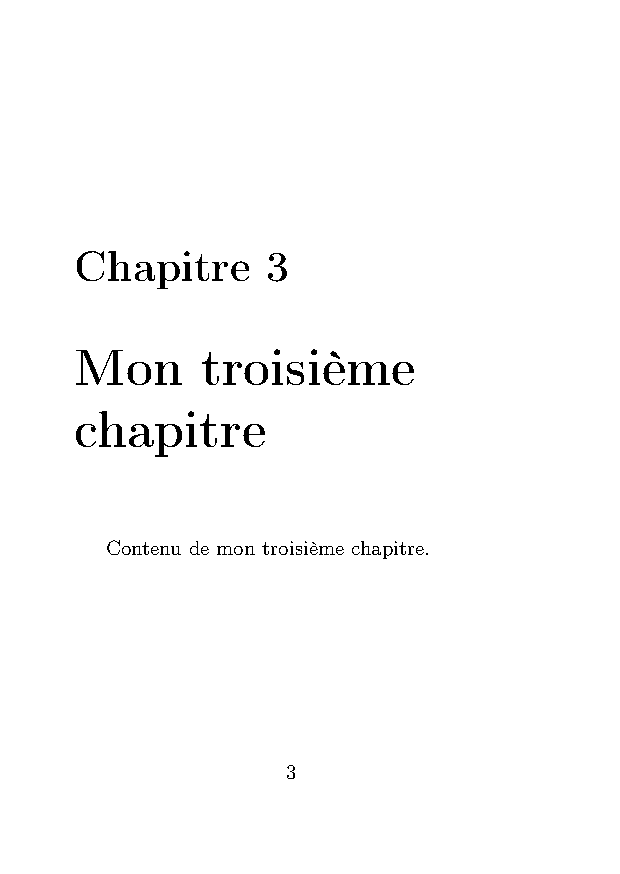
\includegraphics[scale=.5]{images/choix_extensions_exemple_principal}
\end{boxedminipage}





\section[Versions d'un document]{Différentes versions d'un même document}

Pour faire différentes versions d'un même document, utiliser la \emphdef{compilation conditionnelle} avec l'extension \mintinline{latex}{optional}.

Par exemple, pour une compilation destinée uniquement aux élèves, on appelle l'extension \mintinline{latex}{optional.sty} avec l'option \mintinline{latex}{eleves} dans le préambule : \mintinline{latex}{\usepackage[eleves]{optional}}. Puis, dans le fichier, on place les parties uniquement destinées aux élèves dans les deuxièmes accolades d'une commande \mintinline{latex}{\opt{eleves}{}}.

\begin{minipage}{.6\linewidth}
	\begin{minted}{latex}
\documentclass[twoside]{report}
\usepackage[eleves]{optional}

\begin{document}
  \opt{eleves}{cf. formulaires p. 92}} :
  \[
    1+\frac{1}{1!}+\frac{1}{2!}+\dots = \opt{prof}{e}
   \]
\end{document}
	\end{minted}
\end{minipage}
\hfill
\begin{boxedminipage}{.35\linewidth}
	cf. formulaires p. 92 :
	\[
		1+\frac{1}{1!}+\frac{1}{2!}+\dots =
	\]
\end{boxedminipage}

Le même fichier peut contenir une variante pour les professeurs. Dans ce cas, il faut appeler \mintinline{latex}{optional} avec \newline \mintinline{latex}{usepackage[prof]{optional}} dans le préambule et placer le code destiné aux professeurs dans le deuxième argument d'une commande \mintinline{latex}{\opt{prof}{}}.

\begin{minipage}{.6\linewidth}
	\begin{minted}{latex}
\documentclass[twoside]{report}
  \usepackage[prof]{optional}

  \begin{document}
  \opt{eleves}{cf. formulaires p. 92}} :
  \[
    1+\frac{1}{1!}+\frac{1}{2!}+\dots = \opt{prof}{e}
  \]
\end{document}
	\end{minted}
\end{minipage}
\hfill
\begin{boxedminipage}{.35\linewidth}
	\[
		1+\frac{1}{1!}+\frac{1}{2!}+\dots = e
	\]
\end{boxedminipage}

\remarque*{
	Cette pratique est dangereuse pour vos informations : il est facile de se tromper et de transmettre une version du document aux mauvaises personnes. Pour éviter ceci, il est recommandé de créer une copie du document principal pour chaque version, ayant chacune son option pour \mintinline{latex}{\uespackage[...]{optional}}.
}



\section{Insérer une licence Creative Commons}

Pour commencer, il faut choisir sa licence sous \url{http://creativecommons.org/choose/}, par exemple by-nc-as (Creative Commons Attribution - Pas d'Utilisation Commerciale - Partage dans les Mêmes Conditions).

Sur le site de Creative Commons, récupérer la phrase à faire figurer dans le document; ici : "Cette {\oe}uvre est mise à disposition selon les termes de la \href{http://creativecommons.org/licenses/by-nc-sa/3.0/ch/deed.fr}{licence Creative Commons Attribution - Pas d'Utilisation Commerciale - Partage dans les Mêmes Conditions 3.0 Suisse (CC BY-NC-SA 3.0 CH)}".

Eventuellement, récupérer l'image correspondant à la licence, ici : 
\includegraphics[height=2ex]{images/licence_CC_BY_NC_SA}, ou utiliser les commandes de l'extension \href{http://mirror.ctan.org/fonts/ccicons/ccicons.pdf}{\mintinline{latex}{ccicons}} :
\begin{LTXexample}[pos=o,width=.15]
\ccLogo, \ccAttribution, \ccNonCommercial, \ccShareAlike
\end{LTXexample}

Dans le fichier \mintinline{latex}{styles_document.sty}, dans la première section du document, il faut copier la phrase et l'URL de la licence dans la première partie du document, par exemple :	
\begin{minted}{latex}
\hypersetup{
  pdftitle={Choix de l'extension LaTeX pour le collège},
  pdfsubject={Trucs & astuces pour gagner en efficacité et en portabilité},
  pdfkeywords={LaTeX} {Collège} {college} {trucs} {astuces} {efficacité} {portabilité}
    {package}{exemple},
  pdfauthor={Samuel Vannay},
  %Pour insérer une licence Creative Commons (machine readable) dans le fichier pdf
  pdfcopyright={Cette oeuvre est mise à disposition selon les termes de la Licence 
    Creative Commons Attribution - Pas d'Utilisation Commerciale - Partage dans les
    Mêmes Conditions 3.0 Suisse (CC BY-NC-SA 3.0 CH)},
  pdflicenseurl={http://creativecommons.org/licenses/by-nc-sa/3.0/ch}
}
\end{minted}

De cette manière, le fichier pdf contient toutes les informations, lisibles par n'importe qui, mais aussi lisibles par les moteurs de recherches.